\documentclass[12pt,a4paper]{article}
\usepackage[utf8]{inputenc}
\usepackage{amsmath}
\usepackage{amssymb}
\usepackage{graphicx}
\usepackage{hyperref}
\usepackage{booktabs}
\usepackage{float}
\usepackage{enumitem}
\usepackage{geometry}
\usepackage{microtype}
\usepackage{algorithm}
\usepackage{algorithmic}
\usepackage{pgfplots}
\pgfplotsset{compat=1.18}
\usepackage{pifont}
\usepackage{textcomp}
\usepackage[skip=10pt plus1pt, indent=40pt]{parskip}
\setlength{\parindent}{0pt}

\geometry{margin=1in}

\newcommand{\cmark}{\ding{51}}
\newcommand{\xmark}{\ding{55}}
\newcommand{\pmark}{$\sim$}
\newcommand{\lmark}{\textcircled{\scriptsize L}}

\title{\bf ADSP Tutorial: \\Inference Engine}

\author{Vincent Octavian Tiono}
\date{b11901123}

\begin{document}

\maketitle

\begin{abstract}
Inference engines are computational systems that derive logical conclusions from structured data and knowledge bases, serving as the core reasoning backbone for AI systems across domains from natural language processing to medical diagnosis.

Their evolution spans three key eras: rule-based expert systems of the 1970s using forward and backward chaining (MYCIN, OPS5), statistical learning integration in the 2000s adding probabilistic reasoning (Prolog, CLIPS), and modern neural inference engines optimized for large language models and semantic web applications with advanced transformer architectures.

Contemporary inference engines are central to AI infrastructure, powering applications from semantic web reasoning to large-scale language model deployment. The AI inference market is projected to grow from \$89.19 billion in 2024 to \$520.69 billion by 2030, supporting real-time inference for interactive chatbots, decision support systems, and edge computing across healthcare, automation, and IoT networks.

Modern engines employ sophisticated optimization techniques including quantization (up to 75\% memory reduction), key-value caching, and speculative decoding (2–3× speedup). They also leverage advanced batching, parallelization frameworks, and memory-efficient attention mechanisms like PagedAttention and FlashAttention, achieving up to fivefold throughput improvements.

Despite advances, challenges persist, including memory bottlenecks, accuracy-efficiency trade-offs, and hardware compatibility issues. The field is evolving toward hardware-software co-design, dynamic multi-modal inference, distributed reasoning, and sustainable computing, with future developments integrating neuromorphic computing, quantum-classical hybrid systems, and federated inference networks while emphasizing energy efficiency as AI deployment scales globally.
\end{abstract}

\newpage
\tableofcontents
\newpage

\section{Introduction}
\subsection{Inference Engine Fundamentals}
Inference engines are the computational backbone of reasoning systems, allowing machines to use structured algorithmic processes to arrive at logical conclusions. From semantic web applications to large-scale language model serving systems, these engines, first developed for expert systems in the 1970s, have evolved into essential components of contemporary artificial intelligence infrastructure.

An inference engine's primary function is to derive new facts or conclusions from a knowledge base by applying logical rules. This procedure, which is codified using propositional and predicate logic, allows automated reasoning in a variety of fields, including natural language comprehension and medical diagnosis.

\subsection{Historical Evolution and Paradigm Shifts}
The advancement of inference engines spans different technological eras, each characterized by distinct computational paradigms and optimization techniques.

\textbf{Classical Rule-Based Era (1970s-1990s)}: During this foundational period, fundamental reasoning mechanisms were established through forward and backward chaining algorithms. Groundbreaking systems such as MYCIN and OPS5 demonstrated the feasibility of rule-based expert systems for complex decision-making tasks. The basic inference rule was used by these systems:

\begin{equation}
\text{IF } P_1 \wedge P_2 \wedge \ldots \wedge P_n \text{ THEN } Q
\end{equation}

where premises $P_i$ must be satisfied to conclude $Q$, with computational complexity $O(r \times f)$ for $r$ rules and $f$ facts. While naive implementations faced combinatorial challenges, breakthroughs like the Rete algorithm (1982) dramatically optimized pattern matching, enabling practical deployment in commercial systems like CLIPS and later Drools.

\textbf{Machine Learning Integration Period (1990s-2010s)}: This period witnessed the integration of statistical learning techniques with logical reasoning. More robust handling of uncertain information was made possible by the integration of probabilistic reasoning capabilities into systems such as Prolog and CLIPS. This period also saw rule engines transition from academic prototypes to industrial tools, focusing on maintainability and scalability for business rules management.

\textbf{Modern LLM and Semantic Web Optimization (2010s-Present)}: Modern inference engines primarily focus on semantic web reasoning and transformer architecture optimization. Real-time large language model serving is made possible by the attention mechanism implemented by advanced systems such as TensorRT-LLM and vLLM.

\subsection{Computational Foundations and Mathematical Frameworks}
Modern inference engines operate on diverse mathematical foundations. Transformer-based inference engines employ the following fundamental attention mechanism:

\begin{equation}
\text{Attention}(Q,K,V) = \text{softmax}\left(\frac{QK^T}{\sqrt{d_k}}\right)V
\end{equation}

where $Q$, $K$, and $V$ represent query, key, and value matrices respectively, with computational complexity $O(n^2d)$ for sequence length $n$ and dimension $d$.

\textbf{Multi-Query Attention Optimization}: Modern engines use Multi-Query Attention (MQA), which lowers the key and value dimensions, to alleviate memory bottlenecks:

\begin{equation}
\text{MQA}(Q,K,V) = \text{softmax}\left(\frac{QK^T}{\sqrt{d_k}}\right)V, \text{ where } |K|=|V|=1
\end{equation}

This optimization reduces complexity to $O(nd)$ while maintaining comparable accuracy.

\subsection{Market Dynamics and Industry Impact}
The growing adoption of edge computing and generative AI applications is driving unprecedented growth in the inference engine market, as shown in Figure~\ref{fig:ai_inference_market_growth}. North America leads the market with a 36.6\% share, mostly due to significant investments in AI infrastructure made by cloud providers and IT companies.

Key market drivers include:
\begin{itemize}
    \item \textbf{GPU Performance Enhancements}: Advanced hardware acceleration enabling real-time inference at scale
    \item \textbf{Edge Computing Adoption}: Deployment of inference capabilities at network edges for low-latency applications
    \item \textbf{Generative AI Integration}: Widespread adoption of large language models requiring optimized inference infrastructure
\end{itemize}

\begin{figure}[h]
    \centering
    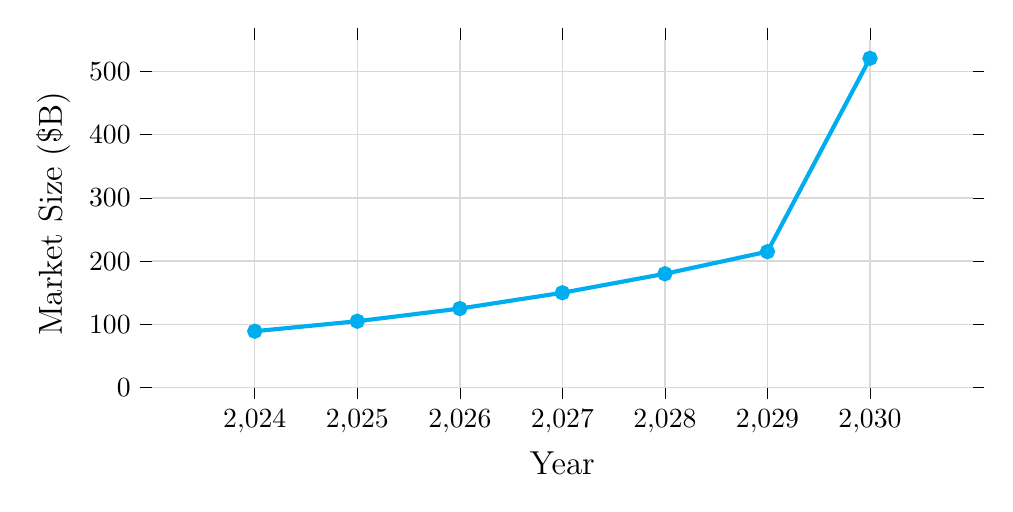
\begin{tikzpicture}
        \begin{axis}[
            xlabel={Year},
            ylabel={Market Size (\$B)},
            ymin=0, ymax=550,
            xmin=2023, xmax=2031,
            xtick={2024,2025,2026,2027,2028,2029,2030},
            ytick={0,100,200,300,400,500},
            grid=major,
            width=12cm,
            height=6cm,
            tick align=outside,
            tick style={black},
            major grid style={line width=0.5pt,draw=gray!30},
            axis line style={line width=1pt,draw=none},
            every axis title/.style={at={(0.5,1.05)}, anchor=south},
            label style={font=\large},
            title style={font=\Large\bfseries},
        ]
        \addplot[color=cyan, line width=1.5pt, mark=*, mark options={fill=cyan}] coordinates {
            (2024,89.19)
            (2025,105)
            (2026,125)
            (2027,150)
            (2028,180)
            (2029,215)
            (2030,520.69)
        };
        \end{axis}
    \end{tikzpicture}
    \caption{AI inference market growth projection showing exponential growth from \$89.19B in 2024 to \$520.69B by 2030 with a CAGR of 19.3\%}
    \label{fig:ai_inference_market_growth}
\end{figure}


\section{Implementation Architectures and Algorithmic Strategies}
\subsection{Classical Inference Engine Architectures}
Conventional inference engines use either forward chaining (data-driven) or backward chaining (goal-driven) procedures, which are organized approaches to knowledge processing.

\textbf{Forward Chaining Implementation}: This method starts by using the facts that are already known and repeatedly applies inference rules to them until it either achieves the desired outcome or cannot generate any additional facts. Throughout the process, the algorithm keeps track of the facts in working memory and methodically checks the conditions of each rule.

\begin{algorithm}
\caption{Forward Chaining}
\begin{algorithmic}
\STATE Initialize working memory with facts
\WHILE{new facts can be derived}
    \STATE Match rules against current facts
    \STATE Select applicable rules
    \STATE Execute rule consequences
    \STATE Add new facts to working memory
\ENDWHILE
\STATE Return derived conclusions
\end{algorithmic}
\end{algorithm}

The computational complexity for forward chaining is $O(r \times f)$ where $r$ represents the number of rules and $f$ the number of facts in the knowledge base.

\textbf{Backward Chaining Implementation}: This approach finds evidence by working backward from the aim. It navigates the inference network using depth-first search.

\begin{algorithm}
\caption{Backward Chaining}
\begin{algorithmic}
\STATE \textbf{Input:} Knowledge base (rules and facts), query (goal)
\STATE Initialize \emph{goal stack} with the query
\WHILE{goal stack is not empty}
\STATE Pop current goal from the stack
\IF{current goal is known as a fact}
\STATE Mark goal as proven
\ELSIF{there exists a rule whose consequent matches the current goal}
\FOR{each such rule}
\STATE Push all antecedents (conditions) of the rule onto the goal stack
\STATE Attempt to prove all antecedents recursively
\IF{all antecedents are proven}
\STATE Mark current goal as proven
\STATE \textbf{break}
\ENDIF
\ENDFOR
\ELSE
\STATE Goal cannot be proven; \textbf{return} failure
\ENDIF
\ENDWHILE
\IF{all goals are proven}
\STATE \textbf{return} success (query is entailed)
\ELSE
\STATE \textbf{return} failure (query cannot be entailed)
\ENDIF
\end{algorithmic}
\end{algorithm}

An example is the Rete Algorithm, which achieves efficiency by sharing nodes for common conditions, storing partial matches, and propagating only changes, making it well-suited for large rule bases with many overlapping conditions.

\begin{algorithm}
\caption{Rete Algorithm}
\begin{algorithmic}
\STATE \textbf{Input:} Set of rules, set of facts (working memory)
\STATE Build the Rete network:
\STATE \quad Create root node
\FOR{each rule}
\STATE Decompose rule conditions into patterns
\STATE Add nodes for each unique pattern (sharing nodes where possible)
\STATE Connect nodes to reflect condition structure (alpha and beta nodes)
\STATE Link leaf nodes to corresponding rule actions
\ENDFOR
\STATE Insert facts into the network:
\FOR{each fact}
\STATE Propagate fact from root node through alpha nodes (simple condition tests)
\STATE Store matches at each node
\STATE At beta nodes, join partial matches from different patterns
\STATE If all conditions for a rule are satisfied at a leaf node, activate (fire) the rule
\ENDFOR
\STATE When facts are added, modified, or retracted:
\STATE \quad Update only affected nodes and propagate changes through the network
\STATE \quad Remove invalidated partial matches as needed
\STATE Repeat propagation as new facts are asserted or existing facts are retracted
\STATE \textbf{Output:} Set of activated rules and their actions
\end{algorithmic}
\end{algorithm}

\newpage

\subsection{Modern Neural Network Inference Architectures}
Contemporary inference engines for neural networks, particularly large language models, implement sophisticated optimization strategies to manage computational and memory constraints.

\textbf{Transformer Inference Architecture}: Modern LLM utilize optimized transformer implementations with attention mechanisms. The core architecture includes:

\begin{enumerate}
    \item \textbf{Input Processing}: Tokenization and embedding layers convert text to numerical representations
    \item \textbf{Attention Computation}: Multi-head attention mechanisms process contextual relationships
    \item \textbf{Feed-Forward Networks}: Position-wise transformations enhance representation
    \item \textbf{Output Generation}: Autoregressive decoding produces sequential outputs
\end{enumerate}

\textbf{Mobile Neural Network (MNN) Architecture}: MNN represents a universal inference engine optimized for mobile deployment. Key innovations include:

\begin{itemize}
    \item \textbf{Pre-inference Optimization}: Runtime optimization through cost evaluation and scheme selection
    \item \textbf{Kernel Optimization}: Optimized operators utilizing improved algorithms and data layouts
    \item \textbf{Backend Abstraction}: Hybrid scheduling while maintaining lightweight deployment (400-600KB binary size)
\end{itemize}

\subsection{Optimization Techniques and Performance Enhancements}
Modern inference engines employ multiple optimization strategies to address the computational challenges of large-scale models.

\textbf{Quantization Strategies}: Model quantization reduces memory footprint and computational requirements while maintaining accuracy. Common approaches include:

\begin{itemize}
    \item \textbf{FP16 Quantization}: 16-bit floating point representation reducing memory by $\sim$50\%
    \item \textbf{INT8 Quantization}: 8-bit integer quantization achieving 75\% memory reduction with minimal accuracy loss
    \item \textbf{Advanced Techniques}: AWQ (Activation-aware Weight Quantization) and other adaptive methods
\end{itemize}

\textbf{KV Caching Optimization}: Key-Value caching eliminates redundant computations in autoregressive generation:

\begin{align}
K_{\text{cached}} &= \text{concat}(K_{\text{prev}}, K_{\text{new}}) \\
V_{\text{cached}} &= \text{concat}(V_{\text{prev}}, V_{\text{new}})
\end{align}

This technique achieves 300\% speed improvement with zero accuracy loss while requiring additional memory proportional to sequence length.

\textbf{Speculative Decoding}: This technique generates multiple tokens simultaneously through parallel speculation:

\begin{equation}
P(x_{t+k}|x_1,\ldots,x_t) = \prod_{i=1}^{k} P(x_{t+i}|x_1,\ldots,x_{t+i-1})
\end{equation}

Speculative decoding achieves 2-3x speedup for text generation while maintaining identical output quality.

\begin{figure}[h]
    \centering
    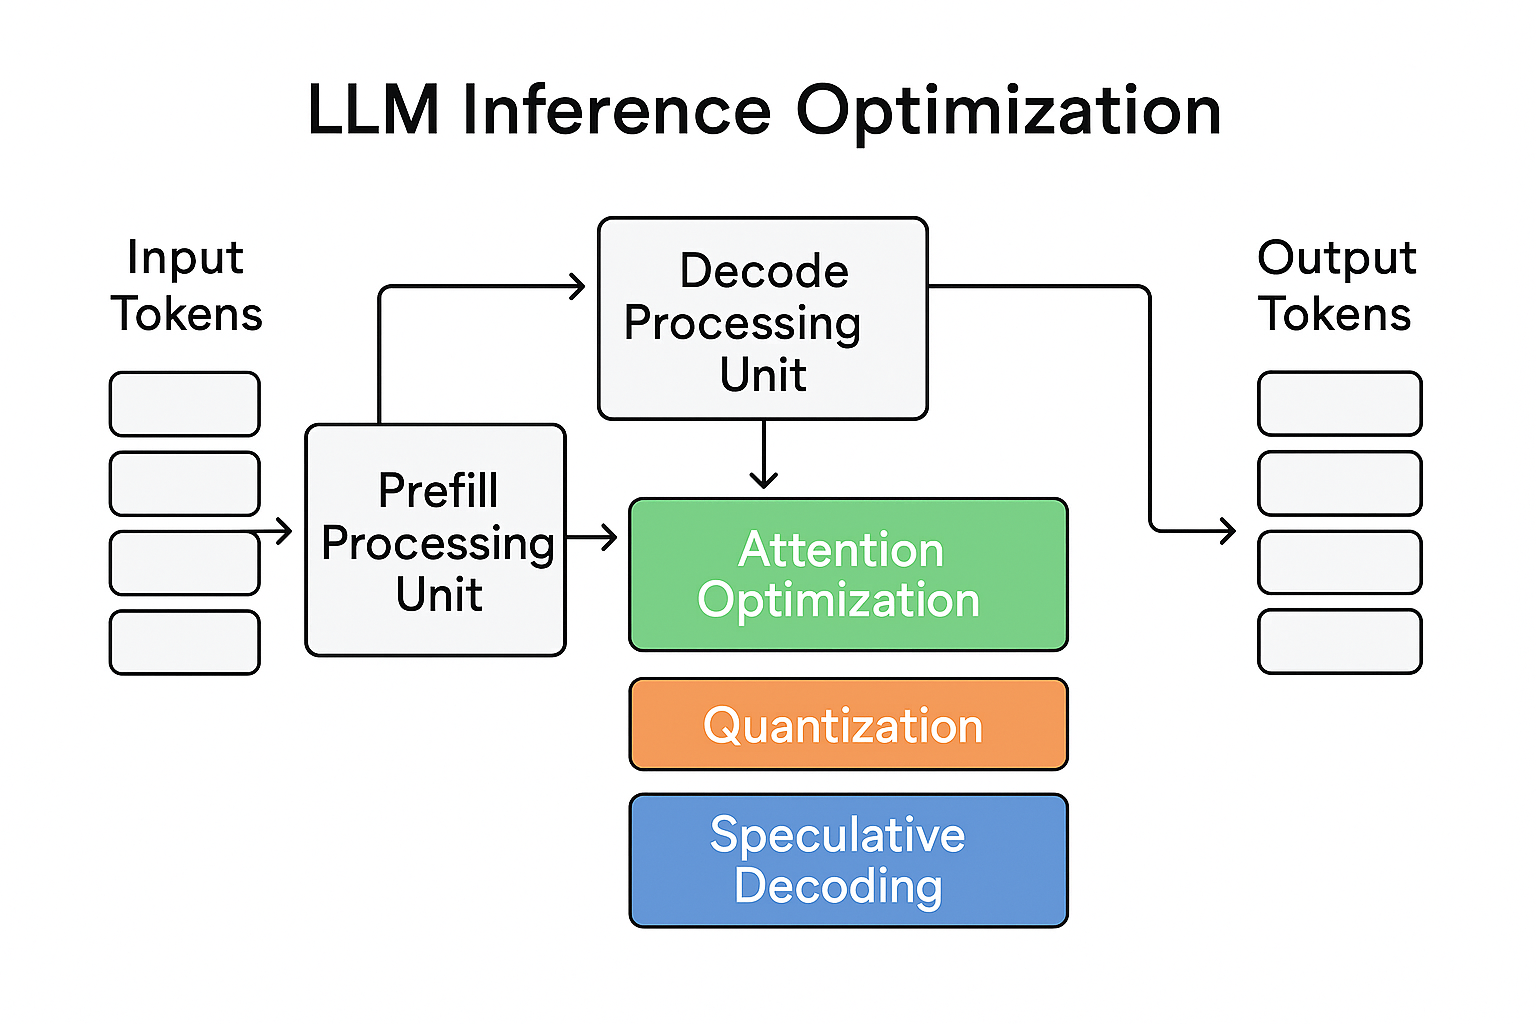
\includegraphics[width=0.8\textwidth]{llm_inference.png}
    \caption{Modern LLM Inference Optimization Techniques showing KV caching, attention optimization, quantization, and speculative decoding}
    \label{fig:inference_market}
\end{figure}

\subsection{Distributed and Edge Inference Systems}
\textbf{Edge Inference Optimization}: Edge deployment requires specialized optimizations for resource-constrained environments. Key strategies include:

\begin{itemize}
    \item \textbf{Model Compression}: Reducing model size through pruning and distillation
    \item \textbf{Hardware-Specific Optimization}: Leveraging specialized accelerators (NPUs, DSPs)
    \item \textbf{Dynamic Inference}: Adaptive computation based on input complexity
\end{itemize}

\textbf{Collaborative Inference Framework}: The Mixture-of-Edge-Experts approach optimizes inference across heterogeneous devices. This framework formulates joint gating and expert selection problems to optimize performance under energy and latency constraints.

\section{Large Language Models Inference Engine }

This section provides an in-depth analysis based on the seminal survey by Park et al. \cite{park2025}, ``A Survey on Inference Engines for Large Language Models: Perspectives on Optimization and Efficiency,'' which represents the most comprehensive evaluation of LLM inference engines to date. The survey systematically examines 25 open-source and commercial inference engines across multiple dimensions, providing critical insights for researchers and practitioners in the field.

\subsection{Survey Scope and Methodology}

\cite{park2025}'s survey addresses a significant gap in the literature by adopting a framework-centric perspective, systematically categorizing LLM inference engines and their optimization techniques. Unlike previous surveys that focused on specific optimization methods, this work provides a holistic view of the inference engine ecosystem, examining each engine across six key dimensions:

\begin{itemize}
    \item \textbf{Ease-of-Use}: Installation simplicity, documentation quality, and developer experience
    \item \textbf{Ease-of-Deployment}: Configuration requirements and production readiness
    \item \textbf{General-Purpose Support}: Model compatibility and architectural flexibility
    \item \textbf{Scalability}: Multi-node and distributed computing capabilities
    \item \textbf{Throughput-Aware Computation}: High-volume batch processing efficiency
    \item \textbf{Latency-Aware Computation}: Real-time and interactive inference optimization
\end{itemize}

The analysis's unique contribution lies in its systematic mapping of optimization techniques to specific inference engines, enabling practitioners to make informed decisions based on their deployment requirements and hardware constraints.

\subsection{Comprehensive Engine Classification}

This analysis categorizes the 25 inference engines across four primary deployment scenarios based on hardware configuration and scaling requirements as shown in Table~\ref{tab:engine_classification}.

\begin{table}[htbp]
\centering
\caption{Classification of LLM Inference Engines by Deployment Scenario}
\label{tab:engine_classification}
\begin{tabular}{@{}p{4cm}p{4cm}p{8cm}@{}}
\toprule
\textbf{Configuration} & \textbf{Scenario} & \textbf{Representative Engines} \\
\midrule
Single-Node, Heterogeneous & Edge/Mobile & Ollama, llama.cpp, MAX, MLC LLM, PowerInfer, TGI \\
\addlinespace
Single-Node, Homogeneous & Specialized & Unsloth, llama2.c, bitnet.cpp, OpenLLM, LightLLM, NanoFlow \\
\addlinespace
Multi-Node, Heterogeneous & Cloud/Hybrid & vLLM, DeepSpeed-FastGen, SGLang, LitGPT, LMDeploy \\
\addlinespace
Multi-Node, Homogeneous & High-Performance & TensorRT-LLM, DistServe, GroqCloud \\
\bottomrule
\end{tabular}
\end{table}

\subsubsection{Engine Performance Analysis}

The survey reveals significant performance variations across different engines, with optimization techniques playing a crucial role in determining throughput and latency characteristics. Table \ref{tab:performance_comparison} presents a comparative analysis of leading engines based on empirical benchmarks.

\begin{table}[htbp]
\centering
\caption{Performance Comparison of Major LLM Inference Engines}
\label{tab:performance_comparison}
\begin{tabular}{@{}lllrrrr@{}}
\toprule
\textbf{Engine} & \textbf{Model} & \textbf{Hardware} & \textbf{Throughput} & \textbf{TTFT} & \textbf{TPOT} & \textbf{Memory} \\
& & & \textbf{(tok/s)} & \textbf{(ms)} & \textbf{(ms)} & \textbf{(GB)} \\
\midrule
vLLM v0.6.0 & Llama 8B & 1x H100 & 1890 & 45 & 8 & 18 \\
TensorRT-LLM & Llama 8B & 1x A100 & 743 & 38 & 12 & 16 \\
Predibase & Llama 7B & 1x H100 & 850 & 42 & 10 & 17 \\
vLLM v0.5.3 & Llama 8B & 1x H100 & 700 & 120 & 40 & 22 \\
DeepSpeed-FastGen & Llama 8B & 1x A100 & 680 & 95 & 35 & 24 \\
Fireworks & Llama 7B & 1x H100 & 650 & 85 & 28 & 19 \\
\bottomrule
\end{tabular}
\end{table}

The performance data demonstrates the substantial impact of optimization techniques, with vLLM v0.6.0 achieving a 2.7x throughput improvement over its previous version through the implementation of chunked prefill and enhanced PagedAttention mechanisms.

\subsection{Optimization Techniques Taxonomy}

This analysis provides a comprehensive taxonomy of optimization techniques implemented across inference engines, categorized into eight primary areas:

\subsubsection{Batch Optimization Strategies}

Modern inference engines employ sophisticated batching techniques to maximize hardware utilization:

\begin{itemize}
    \item \textbf{Dynamic Batching}: Automatically adjusts batch sizes based on available memory and computational resources
    \item \textbf{Continuous Batching}: Enables new requests to join ongoing batches, reducing wait times
    \item \textbf{Nano-batching}: Processes extremely small batches for latency-critical applications
    \item \textbf{Chunked Prefill}: Divides long input sequences into manageable chunks for efficient processing
\end{itemize}

The mathematical formulation for optimal batch size selection is given by:

\begin{equation}
B_{\text{opt}} = \arg\max_B \frac{B \cdot T_{\text{sequence}}}{\text{Latency}(B)}
\end{equation}

where $B$ represents batch size, $T_{\text{sequence}}$ is the average sequence length, and $\text{Latency}(B)$ is the batch-dependent latency function.

\subsubsection{Parallelization Frameworks}

The survey identifies three primary parallelization strategies employed by modern inference engines:

\begin{equation}
\text{Total Speedup} = S_{\text{tensor}} \times S_{\text{pipeline}} \times S_{\text{data}}
\end{equation}

where $S_{\text{tensor}}$, $S_{\text{pipeline}}$, and $S_{\text{data}}$ represent the speedup factors for tensor, pipeline, and data parallelism respectively.

\begin{itemize}
    \item \textbf{Tensor Parallelism}: Distributes individual layer computations across multiple devices
    \item \textbf{Pipeline Parallelism}: Assigns different transformer layers to different devices
    \item \textbf{Data Parallelism}: Replicates the model across devices and distributes input batches
\end{itemize}

\subsubsection{Model Compression Techniques}

The paper analyzes compression methods and their impact on inference performance:

\textbf{Quantization Methods}:
\begin{itemize}
    \item \textbf{Post-Training Quantization (PTQ)}: Achieves 2-4x memory reduction with minimal setup
    \item \textbf{Quantization-Aware Training (QAT)}: Maintains higher accuracy through training-time optimization
    \item \textbf{Advanced Techniques}: AQLM, SmoothQuant, and EXL2 for specialized applications
\end{itemize}

The quantization process can be mathematically represented as:

\begin{equation}
Q(x) = \text{round}\left(\frac{x - Z}{S}\right)
\end{equation}

where $Q(x)$ is the quantized value, $S$ is the scale factor, and $Z$ is the zero-point offset.

\subsection{Optimization Techniques Support Matrix}

Table \ref{tab:optimization_matrix} presents a comprehensive comparison of optimization technique support across major inference engines, revealing significant variations in capability coverage.

\begin{table}[htbp]
\centering
\caption{Optimization Techniques Support Matrix}
\label{tab:optimization_matrix}
\begin{tabular}{@{}p{4cm}ccccc@{}}
\toprule
\textbf{Optimization Technique} & \textbf{vLLM} & \textbf{TensorRT} & \textbf{DeepSpeed} & \textbf{llama.cpp} & \textbf{SGLang} \\
\midrule
Batch Optimization      & \cmark & \cmark & \cmark & \lmark & \cmark \\
Dynamic Batching        & \cmark & \cmark & \cmark & \lmark & \cmark \\
Continuous Batching     & \cmark & \cmark & \cmark & \cmark & \cmark \\
Chunked Prefill         & \cmark & \lmark & \lmark & \lmark & \cmark \\
Tensor Parallelism      & \cmark & \cmark & \cmark & \pmark & \cmark \\
Pipeline Parallelism    & \cmark & \cmark & \cmark & \lmark & \lmark \\
Quantization (INT8)     & \lmark & \cmark & \lmark & \cmark & \lmark \\
Quantization (FP16)     & \cmark & \cmark & \cmark & \cmark & \cmark \\
Quantization (INT4)     & \lmark & \cmark & \lmark & \cmark & \lmark \\
KV Caching              & \cmark & \cmark & \cmark & \cmark & \cmark \\
PagedAttention          & \cmark & \cmark & \lmark & \lmark & \lmark \\
FlashAttention          & \cmark & \cmark & \cmark & \lmark & \cmark \\
Speculative Decoding    & \pmark & \cmark & \lmark & \cmark & \lmark \\
Kernel Fusion           & \cmark & \cmark & \cmark & \lmark & \cmark \\
\bottomrule
\end{tabular}
\end{table}

\textit{Legend}: \cmark = Full Support, \pmark = Partial Support, \lmark = Limited/No Support

\subsection{Attention Mechanism Optimizations}

The research identifies attention optimization as a critical performance factor, with several innovative approaches:

\subsubsection{Memory-Efficient Attention}

\textbf{PagedAttention}: Introduced by vLLM, this technique treats KV cache as virtual memory blocks, enabling dynamic allocation and reducing memory fragmentation. The memory savings can be calculated as:

\begin{equation}
\text{Memory Savings} = \frac{\text{Traditional KV Cache} - \text{Paged KV Cache}}{\text{Traditional KV Cache}} \times 100\%
\end{equation}

Typical savings range from 23\% to 55\% depending on sequence length distribution.

\textbf{FlashAttention}: Optimizes attention computation through memory hierarchy awareness, reducing memory access complexity from $O(N^2)$ to $O(N)$ for sequence length $N$.

\subsubsection{Attention Architecture Variants}

The survey examines the impact of different attention mechanisms on inference efficiency:

\begin{itemize}
    \item \textbf{Multi-Head Attention (MHA)}: Standard approach with full expressiveness
    \item \textbf{Multi-Query Attention (MQA)}: Reduces KV cache by factor of $N_h$ (number of heads)
    \item \textbf{Grouped-Query Attention (GQA)}: Balances between MHA and MQA performance
    \item \textbf{Multi-Head Latent Attention (MLA)}: Compresses KV cache through shared latent vectors
\end{itemize}

The memory reduction factor for GQA is given by:

\begin{equation}
\text{Reduction Factor} = \frac{N_h}{N_g}
\end{equation}

where $N_h$ is the number of heads and $N_g$ is the number of groups.

\subsection{Ecosystem Maturity and Commercial Considerations}

The survey provides valuable insights into ecosystem maturity through analysis of development activity, community support, and commercial viability:

\subsubsection{Open Source Engine Analysis}

Key factors for ecosystem maturity include:

\begin{itemize}
    \item \textbf{Development Velocity}: Commit frequency and feature implementation rate
    \item \textbf{Community Engagement}: Issue resolution time and contributor diversity
    \item \textbf{Documentation Quality}: Completeness and maintenance of documentation
    \item \textbf{Hardware Support}: Breadth of supported platforms and accelerators
\end{itemize}

\subsubsection{Commercial Engine Evaluation}

The survey examines commercial offerings across multiple dimensions:

\begin{table}[htbp]
\centering
\caption{Commercial Inference Engine Comparison}
\label{tab:commercial_engines}
\resizebox{\textwidth}{!}{
  \begin{tabular}{@{}p{4cm}p{4cm}p{4cm}p{4cm}@{}}
  \toprule
  \textbf{Engine} & \textbf{Pricing Model} & \textbf{Key Advantage} & \textbf{Target Market} \\
  \midrule
  Fireworks AI & Pay-per-token & Custom hardware optimization & High-throughput applications \\
  GroqCloud & Subscription & Purpose-built LPU architecture & Real-time inference \\
  Together Inference & Usage-based & Distributed scale & Enterprise deployment \\
  Friendli Engine & Managed service & Optimized model serving & Production-ready solutions \\
  \bottomrule
  \end{tabular}
}
\end{table}


\subsection{Future Directions and Emerging Challenges}

The survey identifies several critical areas for future research and development:

\subsubsection{Hardware Acceleration Trends}

\begin{itemize}
    \item \textbf{Specialized ASICs}: Custom silicon designed specifically for transformer inference
    \item \textbf{Neuromorphic Computing}: Brain-inspired architectures for energy-efficient inference
    \item \textbf{Quantum-Classical Hybrid}: Leveraging quantum advantages for specific inference operations
\end{itemize}

\subsubsection{Algorithmic Innovations}

\begin{itemize}
    \item \textbf{Adaptive Inference}: Dynamic computation allocation based on input complexity
    \item \textbf{Multi-Modal Integration}: Unified optimization for text, image, and audio processing
    \item \textbf{Federated Inference}: Distributed computation across edge devices while preserving privacy
\end{itemize}

\subsubsection{Security and Privacy Considerations}

The survey emphasizes growing concerns around:

\begin{itemize}
    \item \textbf{Model Extraction Attacks}: Protecting proprietary model parameters during inference
    \item \textbf{Data Privacy}: Ensuring input confidentiality in cloud-based inference
    \item \textbf{Adversarial Robustness}: Maintaining performance under malicious input perturbations
\end{itemize}

\subsection{Practical Implementation Guidelines}

Based on the survey findings, we provide actionable recommendations for inference engine selection:

\subsubsection{Use Case-Specific Recommendations}

\begin{table}[htbp]
\centering
\caption{Inference Engine Selection Guide by Use Case}
\label{tab:commercial_engines}
\resizebox{\textwidth}{!}{
    \begin{tabular}{@{}p{6cm}p{6cm}p{6cm}p{6cm}@{}}
    \toprule
    \textbf{Use Case} & \textbf{Primary Requirements} & \textbf{Recommended Engines} \\
    \midrule
    Interactive Chatbots & Low latency, real-time response & vLLM, TensorRT-LLM, GroqCloud \\
    \addlinespace
    Batch Processing & High throughput, cost efficiency & DeepSpeed-FastGen, Together Inference \\
    \addlinespace
    Edge Deployment & Memory efficiency, CPU support & llama.cpp, MLC LLM, PowerInfer \\
    \addlinespace
    Research & Flexibility, model support & SGLang, LitGPT, OpenLLM \\
    \addlinespace
    Enterprise Production & Reliability, managed service & Fireworks AI, Friendli Engine, MAX \\
    \bottomrule
    \end{tabular}
}
\end{table}

\newpage
\subsubsection{Performance Optimization Workflow}

The survey recommends a systematic approach to inference optimization:

\begin{enumerate}
    \item \textbf{Baseline Establishment}: Measure initial performance with minimal optimizations
    \item \textbf{Bottleneck Identification}: Profile computational and memory usage patterns
    \item \textbf{Incremental Optimization}: Apply techniques in order of expected impact
    \item \textbf{Validation and Monitoring}: Ensure accuracy preservation and system stability
\end{enumerate}

\subsection{Conclusion and Impact Assessment}

\cite{park2025}'s survey offers a major contribution to LLM inference optimization, evaluating 25 engines across to provide unprecedented insights into current capabilities and future trends. Key findings include:

\begin{itemize}
    \item \textbf{Performance Gains}: Modern optimization techniques achieve 2-5x improvements in throughput and latency as shown in Figure~\ref{fig:throughput_comparison}
    
    % \item \textbf{Ecosystem Fragmentation}: Significant variation in optimization support requires careful engine selection
    \item \textbf{Hardware Dependency}: Optimal performance increasingly requires hardware-specific optimizations
    \item \textbf{Trade-off Complexity}: Balancing accuracy, performance, and resource utilization remains challenging
\end{itemize}

The survey's framework enables systematic inference engine comparison, addressing critical researcher and practitioner needs in the evolving LLM deployment paradigm.

\begin{figure}[htbp]
\centering
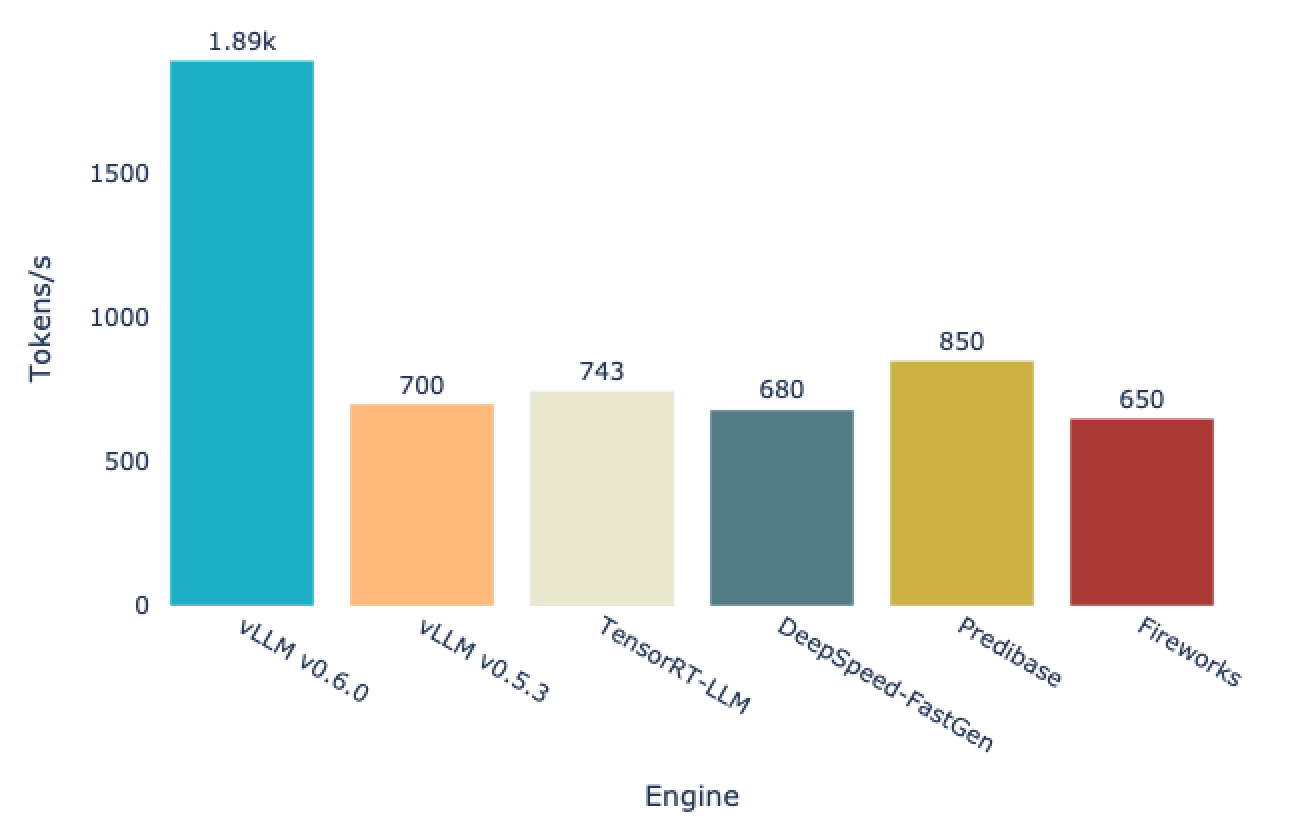
\includegraphics[width=\textwidth]{llm_comparison.png}
\begin{figure}
    \centering
    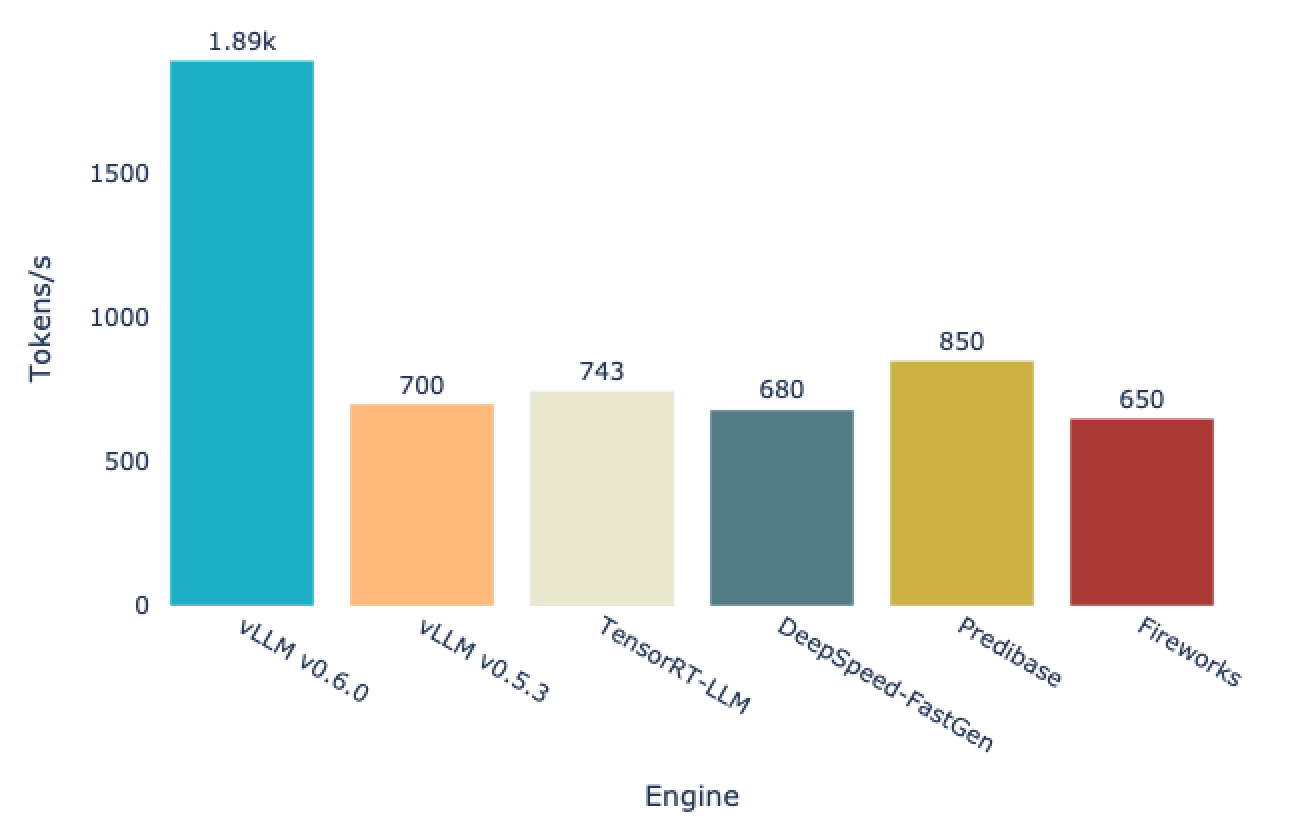
\includegraphics[width=\linewidth, height=9cm, keepaspectratio]{llm_comparison.png}
    \caption{Throughput comparison of major LLM inference engines showing significant performance variations across different optimization approaches}
\label{fig:throughput_comparison}
\end{figure}
\end{figure}

\section{Other Applications Across Domains}

\subsection{Semantic Web and Knowledge Graph Reasoning}

Semantic web and knowledge graph frameworks perform automated reasoning over structured, linked data using standards like RDF, OWL, and SPARQL. They underpin semantic AI applications such as intelligent search, entity linking, and knowledge discovery.

\textbf{Ontology-Based Reasoning:} Modern inference engines for the semantic web perform automated reasoning over ontologies, deriving implicit knowledge through logical entailment. Core reasoning tasks include:

\begin{itemize}
    \item \textbf{RDFS Reasoning:} Implements schema-level inference, including class subsumption, property inheritance, and domain/range constraints. Engines such as Apache Jena and RDF4J provide built-in support for RDFS closure computation.
    \item \textbf{OWL Reasoning:} Facilitates expressive description logic-based reasoning, enabling equivalence, disjointness, and property restrictions. Prominent OWL reasoners include Pellet, HermiT, and FaCT++, supporting OWL DL and OWL 2 profiles (EL, QL, RL) optimized for different computational complexities.
    \item \textbf{Rule-Based Inference:} Extends declarative reasoning with domain-specific rules using syntaxes like SWRL (Semantic Web Rule Language) or custom forward/backward chaining rule engines. Frameworks such as BaseVISor and Euler YAP Engine provide integrated rule-based reasoning environments.
\end{itemize}

\textbf{Deductive Closure and Frame-Based Systems:} F-OWL is a frame-logic inference system that computes ontology entailment through deductive closure, combining forward and backward reasoning via XSB and Flora-2 to support recursive and meta-level inference.

\textbf{Knowledge Graph Reasoning Architectures:} Contemporary reasoning architectures extend beyond description logic, adopting hybrid neuro-symbolic methods and knowledge graph embeddings to manage large, incomplete, and noisy graph data. Techniques include:

\begin{itemize}
    \item \textbf{Path-Based Reasoning:} Utilizes traversal-based algorithms to infer relational paths and transitive closures.
    \item \textbf{Rule Learning:} Applies statistical relational learning (SRL) or differentiable rule mining (e.g., Neural LP, DRUM) to induce inference patterns from data.
    \item \textbf{Embedding-Based Reasoning:} Maps entities and relations to continuous vector spaces using models such as TransE, RotatE, and ComplEx, enabling approximate reasoning via vector arithmetic.
\end{itemize}

\textbf{Performance and Scalability Considerations:} Benchmarks reveal notable performance differences among semantic web reasoners, especially with large knowledge bases and complex rules. Systems like RDFox and GraphDB support parallel reasoning, while frameworks like SANSA Stack use Spark for scalable, distributed inference.

\textbf{Emerging Trends:} The fusion of symbolic reasoning and neural learning is driving neuro-symbolic frameworks like KGAT and R-GCN, enabling scalable reasoning over heterogeneous, incomplete data beyond classical logic systems. 

Semantic web and knowledge graph reasoning are evolving into hybrid, context-aware architectures combining rule-based, deductive, and inductive methods for complex applications in biomedical, enterprise, and AI domains.

\subsection{Expert Systems and Decision Support}
Classical inference engines continue to serve critical roles in expert systems across multiple domains.

\textbf{Medical Diagnosis Systems}: Rule-based inference engines support clinical decision-making through:
\begin{itemize}
    \item \textbf{Symptom-Disease Mapping}: Forward chaining from observed symptoms to potential diagnoses
    \item \textbf{Treatment Recommendation}: Backward chaining from desired outcomes to treatment protocols
    \item \textbf{Drug Interaction Checking}: Real-time inference over pharmaceutical knowledge
\end{itemize}

\textbf{Industrial Automation}: Manufacturing systems utilize inference engines for:
\begin{itemize}
    \item \textbf{Process Control}: Real-time reasoning over sensor data and control rules
    \item \textbf{Quality Assurance}: Automated defect detection and classification
    \item \textbf{Predictive Maintenance}: Inference over historical data to predict failures
\end{itemize}

\subsection{Internet of Things and Edge Computing}

Edge inference engines enable distributed, low-latency reasoning within IoT networks by processing data locally, reducing cloud dependency, and preserving privacy.

\textbf{IoT Rule Processing:}  
Forward-chaining engines excel in IoT settings by continuously evaluating real-time sensor data against rule sets to trigger automated actions. Applications include anomaly detection, predictive maintenance, and context-aware control in resource-constrained environments.

\textbf{Distributed Inference Networks:}  
Modern systems implement decentralized reasoning using consensus algorithms (e.g., Paxos, Raft) to ensure consistent decisions across sensor nodes. These architectures achieve $O(k \times \log k)$ complexity for $k$ nodes, supporting coordinated control in smart grids, industrial automation, and autonomous systems.

\textbf{Edge-Cloud Collaborative Inference:}  
Hybrid frameworks partition inference tasks between edge devices and cloud services based on latency, resource availability, and privacy needs. Platforms like AWS Greengrass and Azure IoT Edge enable local rule evaluation with cloud fallback for complex tasks, improving responsiveness and resilience.

In summary, IoT inference systems are evolving toward decentralized, adaptive architectures capable of real-time, context-aware reasoning in dynamic environments.


\section{Limitations and Challenges}
\subsection{Computational Complexity and Scalability}
\textbf{Memory Bottlenecks}: Modern inference engines face significant memory constraints, particularly for large language models. The KV cache grows linearly with sequence length, batch size, and model dimensions, creating substantial memory pressure.

\textbf{Attention Mechanism Limitations}: The quadratic complexity of attention mechanisms poses fundamental scalability challenges:

\begin{equation}
\text{Complexity}_{\text{attention}} = O(n^2 d)
\end{equation}

where $n$ represents sequence length and $d$ the model dimension. This quadratic scaling becomes prohibitive for long sequences.

\textbf{Autoregressive Generation Constraints}: Sequential token generation in language models prevents effective parallelization, limiting throughput in real-time applications.

\subsection{Accuracy and Approximation Trade-offs}
\textbf{Quantization Accuracy Loss}: While quantization techniques achieve substantial memory and speed improvements, they introduce accuracy degradation. INT8 quantization typically results in 2-5\% accuracy loss depending on the model and task.

\textbf{Speculative Decoding Verification}: Although speculative decoding maintains theoretical equivalence to standard generation, practical implementations may introduce subtle differences due to numerical precision and sampling variations.

\textbf{Rule-Based System Brittleness}: Classical inference engines suffer from brittleness when encountering edge cases not explicitly covered by rule sets, requiring comprehensive knowledge engineering.

\subsection{Hardware and Infrastructure Constraints}
\textbf{Edge Device Limitations}: Mobile and edge deployment faces severe resource constraints:
\begin{itemize}
    \item \textbf{Memory Constraints}: Limited DRAM and cache capacity restricting model size
    \item \textbf{Computational Power}: Reduced processing capability compared to datacenter hardware
    \item \textbf{Energy Efficiency}: Battery life considerations requiring power-aware optimization
\end{itemize}

\textbf{Heterogeneous Hardware Challenges}: Supporting diverse hardware architectures (GPUs, TPUs, NPUs) requires extensive optimization and testing across multiple platforms.

\subsection{Integration and Compatibility Issues}
\textbf{Framework Fragmentation}: The growth of inference frameworks creates compatibility challenges, as models often require framework-specific optimizations.

\textbf{Version Management}: Rapid evolution of inference engines creates versioning challenges, particularly for production deployments requiring stability guarantees.

\textbf{Standardization Gaps}: Lack of unified standards for inference optimization techniques complicates cross-platform deployment and performance comparison.

\section{Future Prospects and Emerging Trends}
\subsection{Hardware-Software Co-design Evolution}
\textbf{Neuromorphic Computing Integration}: Future inference engines will leverage neuromorphic hardware architectures that mimic biological neural networks, potentially achieving orders of magnitude improvements in energy efficiency for inference tasks.

\textbf{Quantum-Classical Hybrid Systems}: Emerging quantum computing technologies may enhance specific inference operations, particularly for optimization problems and certain types of search within large knowledge spaces.

\textbf{In-Memory Computing}: Processing-in-memory architectures reduce data movement, addressing memory bottlenecks that limit inference performance.

\subsection{Advanced Optimization Techniques}
\textbf{Dynamic Inference Adaptation}: Future systems will dynamically adapt inference strategies using input features, hardware constraints, and performance objectives.

\textbf{Multi-Modal Inference Integration}: Next-generation engines will seamlessly handle multi-modal inputs (text, images, audio) through unified optimization frameworks.

\textbf{Attention Mechanism Innovations}: Research continues on alternatives to quadratic attention, including:
\begin{itemize}
    \item \textbf{Linear Attention}: Reducing complexity to $O(nd)$ through kernel methods
    \item \textbf{Sparse Attention}: Leveraging structured sparsity patterns to reduce computation
    \item \textbf{Hierarchical Attention}: Multi-scale attention mechanisms for efficient long-sequence processing
\end{itemize}

\subsection{Distributed and Collaborative Inference}
\textbf{Federated Inference Networks}: Distributed inference systems will enable collaborative reasoning across multiple organizations while preserving data privacy.

\textbf{Edge-Cloud Hybrid Architectures}: Intelligent workload distribution between edge and cloud resources will optimize latency, bandwidth, and privacy requirements.

\textbf{Swarm Intelligence Integration}: Multi-agent inference systems will coordinate across networks of devices to solve complex reasoning tasks collaboratively.

\subsection{Sustainability and Efficiency Focus}
\textbf{Green AI Inference}: Environmental considerations will drive development of energy-efficient inference techniques, particularly important as AI deployment scales globally.

\textbf{Carbon-Aware Optimization}: Inference engines will optimize for carbon efficiency, jointly maximizing performance while minimizing environmental impact.

\textbf{Lifecycle Optimization}: Holistic approaches will consider the entire inference pipeline from model training through deployment and maintenance.

\section{Conclusion}
Inference engines have progressed from basic rule-based expert systems to advanced optimization frameworks at the heart of modern AI, reflecting the growing complexity of models and the need for real-time, scalable inference across diverse applications. While traditional forward and backward chaining algorithms remain important for semantic web reasoning and expert systems, contemporary neural inference engines now focus on optimizing transformer architectures with techniques like KV caching, quantization, and speculative decoding to address the computational demands of large language models.

Mathematically, these engines face significant challenges: rule-based systems typically operate with linear complexity, but attention mechanisms in transformers introduce quadratic scaling, which can limit scalability. Innovations such as Multi-Query Attention help reduce this burden, highlighting the ongoing importance of algorithmic improvements for efficient inference.

A comparative analysis of 25 inference engines from \cite{park2025} shows that no single solution is universally best; instead, engine choice should be guided by specific application needs, hardware constraints, and desired optimizations. Leading engines like vLLM, TensorRT-LLM, DeepSpeed, and llama.cpp each excel in different scenarios, from high-throughput cloud environments to resource-constrained edge deployments, with commercial offerings expanding options for enterprise and real-time use.

Despite rapid progress, challenges persist, including memory bottlenecks, trade-offs between efficiency and accuracy, and hardware diversity. The future of inference engines will likely feature tighter hardware-software co-design, dynamic and multi-modal inference, and a focus on sustainability, ensuring these systems continue to drive AI innovation as hybrid architectures that blend symbolic and neural approaches. As AI applications continue to scale globally, inference engines will remain a pivotal focus area, driving both the operational and ethical dimensions of AI deployment.

\renewcommand{\refname}{}
\section{References}
\begin{thebibliography}{99}
\vspace{-1.0cm}
\bibitem{singh2010}
Singh, S., \& Karwayun, R. (2010). A Comparative Study of Inference Engines. \textit{Seventh International Conference on Information Technology: New Generations}, 53-57.

\bibitem{rattanasawad2018}
Rattanasawad, T., Buranarach, M., Saikaew, K. R., \& Supnithi, T. (2018). A Comparative Study of Rule-Based Inference Engines for the Semantic Web. \textit{IEICE Transactions on Information and Systems}, E101-D(1), 82-89.

\bibitem{jiang2020}
Jiang, X., Wang, H., Chen, Y., Wu, Z., Wang, L., Zou, B., Yang, Y., Cui, Z., Cai, Y., Yu, T., Lv, C., \& Wu, Z. (2020). MNN: A Universal and Efficient Inference Engine. \textit{Proceedings of Machine Learning and Systems}, 2020.

\bibitem{park2025}
Park, S., Jeon, S., Lee, C., Jeon, S., Kim, B., \& Lee, J. (2025). A Survey on Inference Engines for Large Language Models: Perspectives on Optimization and Efficiency. \textit{arXiv preprint arXiv:2505.01658}.

\bibitem{zhou2023}
Zhou, Z., Ning, X., Hong, K., Fu, T., Xu, J., Li, S., Lou, Y., Wang, L., Yuan, Z., Li, X., Yan, S., Dai, G., Zhang, X., Dong, Y., \& Wang, Y. (2023). A Survey on Efficient Inference for Large Language Models. \textit{arXiv preprint}.

\bibitem{weng2023}
Weng, L. (2023). Large Transformer Model Inference Optimization. \textit{Lil'Log Blog}.

\bibitem{computerphile_rete}
Computerphile. (2018, July 16). The Rete Algorithm: AI Rule-Based Systems [Video]. \textit{YouTube}. Retrieved from \url{https://www.youtube.com/watch?v=XtT5i0ZeHHE}

\bibitem{wiki_forward}
Forward chaining. \textit{Wikipedia}. Retrieved from \url{https://en.wikipedia.org/wiki/Forward_chaining}

\bibitem{wiki_forward}
Backward chaining. \textit{Wikipedia}. Retrieved from \url{https://en.wikipedia.org/wiki/Backward_chaining}

\bibitem{wiki_rete}
Rete algorithm. \textit{Wikipedia}. Retrieved from \url{https://en.wikipedia.org/wiki/Rete_algorithm}


\end{thebibliography}

\end{document}